%!TEX root = ./Structure_rapport_final.tex


\subsection{Structure and dynamics of ecosystems: how can species coexist in same environment?} 

Of all the questions raised when it comes to study Nature, the most common yet complex one is “how do organisms and environment interact with each other?” \citep{sutherland2013}. In other words, what are the processes and rules that define structure and functioning of ecosystems? Taken as a whole, an ecosystem can be seen as a giant network: all individuals from every species are linked to one another through intra- and inter-specific relationships, that implies competition, parasitism, predation\ldots{}; and each individual is linked to its physical environment, on which it depends for food prospection, shelter and/or favorable conditions for breeding. The main purpose of ecology is to study those links and ultimately, to be able to map the central relationships and flows that are keys to maintain stable ecosystems \citep{albouy2011}. Community ecologists, regardless of the ecosystem they are studying, try to answer some fairly similar questions such as “how do species share environmental resources?” or “how can species relying on the same resource to thrive and survive can coexist?”. Indeed, the mere observation that species can live and develop a population without encroaching each other suggests that, even if species compete to access the same resources, the use of resources is balanced and allows stable relationships between species to develop. Most of all, if species depend on the same resources to survive, how can diversity within an ecosystem last over time?

\subsection{Concepts and definition for studying ecosystems’ dynamic.}
 
To answer those questions, the structure and dynamic of ecosystems need to be investigated and ecological concepts must be defined. \\ First, a ``community'' is made up of all living organisms (all species combined), which interact and occupy a specific habitat. Within this habitat, the concept of ``ecological niche'' reflects the fact that distinct populations use differently space and trophic resources to meet their needs. In 1917, Grinnell was the first to scientifically as ``ecological niche'' all the requirements that a species needs to thrive \citep{grinnell1917}.
This concept covers both biotic (food abundance and availability, competition within and among species, predation-prey relationships \ldots{}) and abiotic conditions (environmental factors such as temperature or pression, shelter availability \ldots{}), and it shapes the areas suited for species according to their needs. This definition is refined by \citet{hutchinson1957}: resources and their availability are the main drivers for the coexistence of species, since resources are essential for species to thrive and are therefore considered limiting factors. Furthermore, Hutchinson’s definition distinguishes the concepts of (i)``fundamental niche'', which is a potential niche for a given species that offers all the optimal conditions for that species to flourish and (ii) ``realized niche'', which corresponds to the actual resources used by a species and which is often smaller than the fundamental niche, mainly because of competition between species. If resources are limited, competition between species that seek to simultaneously exploit the same resources may arise, either because they hunt the same prey or because they live in the same specific habitat and are therefore more likely to meet \citep{blondel1979}. When the resources are abundant enough, species may be able to share it without entering competition \citep{nagelkerke2018}. According to competition theory, community structures are defined by the way species are able to share or not resources. Therefore, to study the structure and dynamics of community and to identify the main factors that enable species to coexist, it is essential to determine the degree by which species share resources, in other words, quantify the overlap between ecological niches \citep{geange2011}. 


\subsection{Tools to study diversity in ecosystems and their limits}

Niche overlap can be approached from the habitat (beta overlap) or food (alpha overlap) perspective \citep{mouillot2005}. In both cases, a high degree of overlap means that the species are likely to compete for the same resources making their coexistence virtually impossible. Conversely, a low deree of overlap tends to suggest that species, even if they rely in part on the same resources, have a sufficiently wide range of accessible resources not to compete with each other \citep{mouillot2005}. No overlap means that species occupy distinct niches, are likely to use very different resources and that no competition is expected (see \ref{fig:lr1}. This approach has been widely developed over the last decades to study the distribution of abundance and the mechanisms favoring species coexistence, in particular to predict the impact of disturbances, such as the introduction of invasive species or climate change \citep{albouy2011,geange2011, martini2020}. 
\begin{figure} [!htbp]
	\begin{center}
		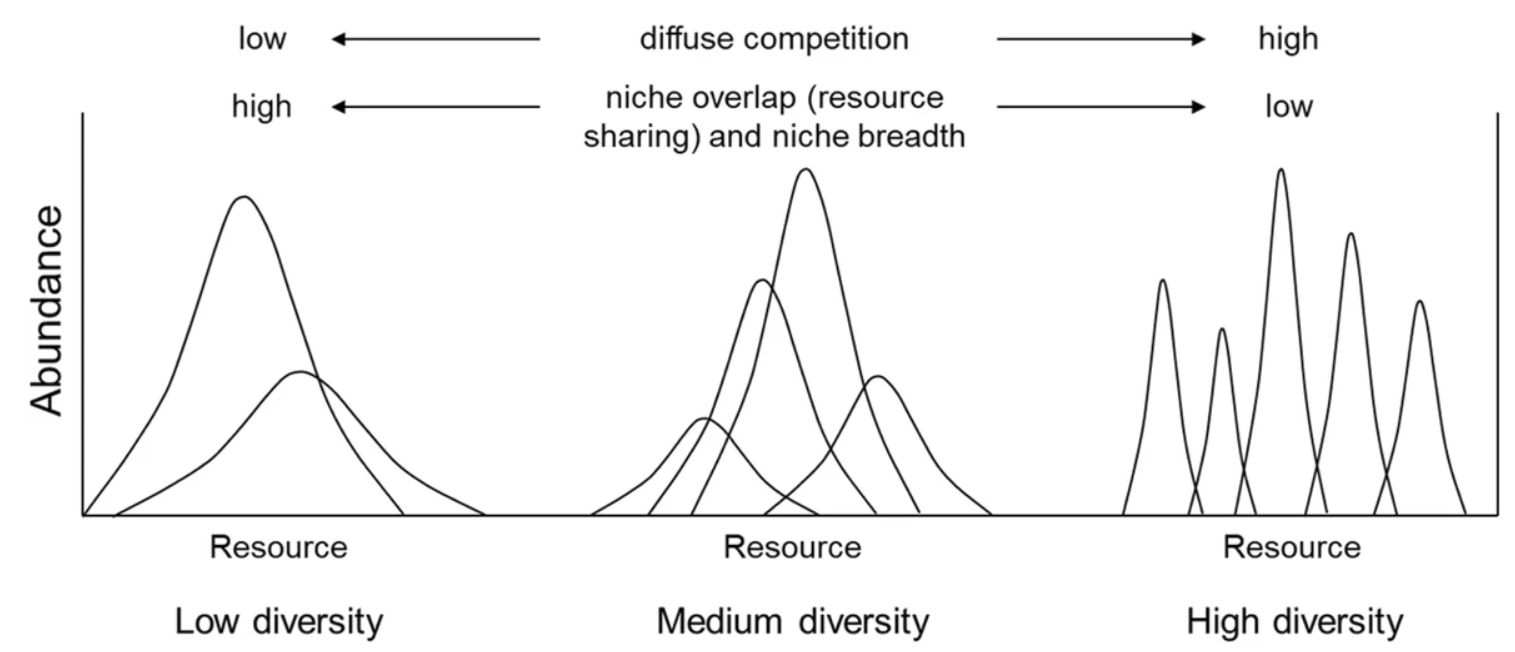
\includegraphics[width=0.8\textwidth]{niche_overlap.png}
	\end{center}
	\caption[Petite légende]{Caracteristics of niches along a resource gradient at different levels of species diversity, from \citet{kim2020}.}
	\label{fig:lr1}
\end{figure}

To quantify niche overlap, several indices have been developed since the 60’s. Indices and threshold values are commonly used for studying specific, taxonomic or phylogenetic diversity. However, used alone, a result of diversity estimation through any index is usually poor and inaccurate, because complex and rich systems can not be described only by the result of a computation \citep{mejri2009}. Indeed, four of the best-known niche overlap indices, which are based on the intensity of utilisation of a resource use by species, were compared by \citet{linton1981} to assess the precision and accuracy: \citet{morisita1959} updated by \citet{horn1966}, \citet{schoener1968} and \citet{pianka1973}. Even if they lead to the same general conclusions, these four indices often give different results, because they use different computation parameters \citep{blondel1979}. Moreover, they are often highly sensitive to sample size, which adds uncertainty when it comes to interpreting their values \citep{linton1981}. Finally, \citet{grossman2009} points out that threshold values for those indices can be considered as arbitrary and might differ from one ecosystem to another, leading to an impossibility of comparing them. For all these reasons, using those indices to estimate if species share or not the same resources, and if so, how much is shared, does not seem relevant \citep{mouillot2005}. As such, they provide a qualitative assessment of the overlap rather than a quantitative one \citep{linton1981}.

Therefore, to understand how the structure and the dynamics of an ecosystem are defined and how such complex relationships can last for several generations, numerical models are often used (see Ecopath models, \url{https://ecopath.org}). This approach requires a simplification of the ecosystem, because simulating very complex models make the outcome virtually impossible to compute \citep{albouy2011}. Simplifying an ecosystem can be done in many ways: focusing on specific compartments of the ecosystem (\textit{e.g}: pelagic or benthic fauna), grouping species based on their trophic level, or taxonomy or similaire behavior \ldots{}. Obviously, simplifying with any of these methods comes down to approximating the relationships and much of the complexity of an ecosystem, but if done properly, models are still able to produce reliable simulations of what is going on in real life \citep{albouy2011,evans2012,piroddi2015}. Yet, the main difficulty is to determine the criteria that are relevant to gather species and to simplify models. Whether they are too restrictive, or not enough, these criteria condition not only the accuracy of the model, but also its ability to be generalized \citep{moon2017,pease2015,pont2006}. For instance, if a model uses a taxonomic grouping of species, it will only be suited to study other ecosystems that contain the ame set of species or taxonomic groups. Its transposition to other unrelated ecosystems will thus be limited, if not impossible \citep{moon2017}. In the end, this modeling approach imposes a specific model for each ecosystem, which is highly time consuming and limits the possibilities of comparisons between ecosystems \citep{martini2020, mcgill2006}. Therefore, this approach remains very specific to a studied ecosystem and the species that compose it. 

%How does the morphology of fish impact its behaviour? 
%How can the morphology of the fish help us to understand more about its behaviour?

\subsection{Emergence of a more global approach based on functional traits.}

\subsubsection{General overview}

Community ecology aim to establish general rules explaining the functioning of communities. Species-centred approaches only provide information for a few specific systems but not general principles, that can be applied to a wide variety of communities or ecosystems \citep{albouy2011,martini2020}. Therefore, ecologists had to find a way to study ecosystems, to (i) give clues of how species interacts with each other and (ii) to assess how strongly species are related to their environment. Indeed, some scientists emphasized the urge to get rid of methods that were highly dependent of species, time or space, such as the ones described previously, and to use a more predictable and quantitative science that could play a major role in assessing global changes issues \citep{brindamour2011,mcgill2006,olden2002}. To this extend, \citet{mcgill2006} define a \textbf{trait} as a “well-defined, measurable property of organisms, usually measured at the individual level and used comparatively across species” and suggest that community ecology should try to understand how these traits interact with fundamental niches to define realized niches. The notion of ``trait'' has been widely used in the literature, but with slightly different meanings. For instance, \citet{violle2007} defined a trait as “any morphological, physiological or phenological feature measurable at the individual level, from cell to whole organism”. To ensure a consistent approach to community ecology studies, \citet{martini2020} suggests that the definition of \citet{violle2007} is precise enough, that it should serve as a reference and therefore should be used systematically. Yet, not all measurable traits provide the same information: for ecologists, traits that inform about (i) the interactions between species and the environment and (ii) the fitness of individuals are the most valuables \citep{kremer2017}. These specific traits are defined as “functional traits” and can relate to behavior, life history, morphology or physiology, influencing the general performances of organisms \citet{martini2020, mcgill2006}. They provide information on the main functions of organisms, such as acquisition of food or locomotion \citep{mejri2009}.

\subsubsection{Improvement of the method over the years}
The functional-traits approach was first developed in studies based on terrestrial plants. They showed that the morphology of species was correlated with their environment and that changes in their habitat could lead to changes of their morphology because this approach relies on the plasticity of traits \citep{boissezon2014,lavorel1997,martini2020}. Applied to aquatic animals, structure-function relationship has been well documented since the 1970s \citep{gosline1971, lagler1977, webb1984} and approaches based on morphological traits  seemed suitable to compare species \citep{norton1995} or to explore niches and compare communities \citep{winemiller1991}. For instance, \citet{albouy2011} developped a model to determine the diet of any marine species based on morphological traits, and thus establish trophic guilds. Yet, the model could not predict diet overlap nor resource partitionning among species, because of intrinsic variability in the diet of fish. Indeed, morphology alone is hardly a clue to determine diet, for generalist species are able to switch prey depending on which  is more abundant, and they do not display specific morphological traits \citep{sibbing2000}. \emph{Moreoever, trophic level impacts how specialised a species can be in terms of diet: apex predators will often favor one feeding strategies among others, so they are very efficient for one strategy, and have limitating capacities in others. This principle can be summed up as a ``trade-off strategy'': greater abilities for one strategy lead to a decrease of abilities in other areas \citet{norton1995}, because of morphological specificities \citep{nagelkerke2018}.}

Conversely, when studying morphological trait associated with swimming performances, \citet{webb1984} noticed that most species were not specialized i.e not displaying any particular traits) and had fairly good performances in 3 of the main swimming methods (powerful short acceleration, cruise and maneuvrability). Similarly, using only morphological traits to describe mains functions such as food acquisition does not seem relevant. Indeed, \citet{grossman2009} showed that species with strong morphological divergences sometimes use the same resources in a similar way, whereas morphologically close species can have very different diets. In order to overcome the limits imposed by their morphology and/or habitat for the acquisition of food, organisms can indeed modulate their behavior and show great adaptability \citep{blondel1979,grossman2009}. In fact, if morphology sets limits to resource use, species usually display some plasticity to adapt to prey availability and environmental conditions \citep{ibanez2007,sibbing2000}. The link between morphology and food acquisition is therefore not so robust.

While the flexibility and intrinsic variabiliy of species should not be ignored, they can be hard to predict \citep{diderich2006,martini2020}. It is therefore essential to identify and select relevant traits, that can be used to explain most interactions between species and their environment. This is one of the main challenges of the functional traits approach, because the selected traits must be sufficiently variable beteen the levels being compared (species, populations, individuals …), and the observed variations must explain the actual differences in fitness or coexistence of species \citep{kremer2017}. \\

Yet, the flexibility in traits is what makes this approach so useful, as it allows for the quantification of intraspecific variability (especially when the environmental conditions change \citet{martini2020}) and interspecific variability that explains the interactions between species and their environment. In a nutshell, the traits to be used for functional trait approach must offer the best compromise between being (i) sufficiently informative with respect to the objectives, (ii) generic enough to be comparable across species --- even if they are very different morphologically --- and (iii) easily measurable to ensure repeatability between studies \citep{dumay2004, kremer2017}.

\subsection{The advent of functional diversity}
The functional approach is relatively recent. It developed in the 1980s with the collapse of populations, species extinctions and the biodiversity crisis \citep{wilson1988}. The functions performed by species began to be studied in greater depth when ecologists noticed that if a species disappeared from an ecosystem, it did not necessarily mean that the whole ecosystem was disturbed or even collapsed \citep{mejri2009}. The question ``Are all species essential for the proper functioning of ecosystems?'' became central, as did the need to define the role of species within ecosystems. In other words, can we consider that species are ``redundant" if they play the same role, fulfill the same function, in an ecosystem? To answer these questions, the functional trait approach seems relevant because it provides information on the roles of species in their environment, which is complementary to those provided by classical diversity indices, such as specific diversity, richness distribution or evenness \citep{marcon2015,mejri2009}. 

More importantly, functional traits and species role attribution are crucial in determining functional diversity, which is the primary factor explaining stability and productivity, and should therefore be preferred to specific or taxonomic diversity when studying community ecology \citep{dumay2004,mejri2009}. In fact, the resilience and health of ecosystems depends much more on the range of functions and functional traits exhibited by species than on the number of species \textit{per se} (i.e. species richness). Indeed, indices of specific abundance and diversity assume that all species are equivalent, and do not take into account the functions provided by these species \citep{mejri2009}. From this functional perspective, the richness of an ecosytem is determined by the extent of functional diversity provided by the species \citep{rocklin2004}. 

To estimate functional diversity, species must first be classified into ``functional groups'', which reflects the similarities of species according to 3 criteria. Within a functional group, species must (i) share the same habitat and trophic level \citep{brindamour2016}, (ii) play a similar role in the habitat, through the functions they provide \citep{dumay2004,mejri2009}, and (iii) display similar responses to changing environmental pressures \citep{brindamour2016,dumay2004,mejri2009}.

To form these groups and to evaluate the response of species for each of these 3 items, morphological traits are often used, because they reflect the capacities as well as their modes of interaction with their environment. They can therefore be used as indicators of trophic networks or habitats \citep{brindamour2016}. Indeed, according to the “niche filtering hypothesis”, which considers habitat characteristics as filters, only species that with adapted traits can thrive in a specific set of environmental conditions \citep{brindamour2011}. This assumption also means that species, if they share similar functional traits, must use the same resources, probably in the same way, and thus have overlapping niches. Conversely, if species have very different functional traits from each other, they probably use resources in very different ways, or even distinct resources. 

\subsubsection{Benefits of this approach}

Species in a same functional group can be considered ``functionally equivalent'', with similar or interchangeable functions. The ecosystem in which they occur then has ``functional redundancy'', which reduces the risk of a functional loss in the event of ecosystem disturbance. Conversely, a species can also be the only representative of a functional group (qualified as a ``monospecific group''). It is then considered ``essential'', because if it disappears, the functions it provides will also disappear, causing a major disturbance of the ecosystem and other essential functions \citep{mejri2009}. 

For conservation issues and the prediction of climate change impacts on ecosystems and biodiversity, the functional approach and the study of niche overlap seem relevant, as these tools provide a quantitative estimate of the resilience and/or resistance to change of communities and ecosystems. 
 At a specific level, knowing which species have the most specialised diet or which are the species are essential, from a functional perspective, are really useful to target species that needs to be protected in conservation plans \citep{mejri2009,norton1995}. In addition, those tools can also be used to predict changes in diet niche for species in competition, if one of the abundances is affected by fishing pressure \citep{diderich2006} or if an invasive species colonizes the environment \citep{albouy2011,geange2011,nagelkerke2018}. As these approaches are not based on species or taxonomy, they are better suited to the generalization and identification of the ecosystem services provided \citep{martini2020,mcgill2006} and the relationships involved in stable coexistence of species \citep{albouy2011}. They thus improve our ability to predict ecological dynamics and their fluctuations, in an environment facing strong anthropic influence \citep{kremer2017}. 

+ principe d'exclusion !!!